% =============================================================
%  DAHS -- Elsevier elsarticle  [3p, times, numbered refs]
%  Visual format reference: Mechatronics 104 (2024) 103256
%  Compile order:  pdflatex -> pdflatex -> pdflatex
%  All figures use TikZ / pgfplots -- NO external image files.
%  Tested on Overleaf (pdfLaTeX, TeX Live 2023).
% =============================================================
\documentclass[3p,times]{elsarticle}

%% ---- natbib numbered style ---------------------------------
\biboptions{comma,sort&compress}

%% ---- Language & encoding -----------------------------------
\usepackage[T1]{fontenc}
\usepackage[utf8]{inputenc}

%% ---- Mathematics -------------------------------------------
\usepackage{amsmath}
\usepackage{amssymb}
\usepackage{bm}

%% ---- Graphics & colour -------------------------------------
\usepackage{graphicx}
\usepackage{xcolor}

%% ---- TikZ & pgfplots  (all figures drawn inline) ----------
\usepackage{tikz}
\usepackage{pgfplots}
\pgfplotsset{compat=1.17}
\usetikzlibrary{
  shapes.geometric, arrows.meta, positioning,
  fit, calc, backgrounds, decorations.pathreplacing
}

%% ---- Tables ------------------------------------------------
\usepackage{booktabs}
\usepackage{multirow}
\usepackage{array}
\usepackage{tabularx}

%% ---- Misc --------------------------------------------------
\usepackage{microtype}
\usepackage{url}
\usepackage{lineno}   % \linenumbers -- uncomment for blind review

%% ---- Hyperlinks (matches PDF blue link style) -------------
\usepackage{hyperref}
\hypersetup{
  colorlinks = true,
  linkcolor  = blue!70!black,
  citecolor  = blue!70!black,
  urlcolor   = blue!70!black
}

%% ---- Journal declaration -----------------------------------
\journal{Computers \& Industrial Engineering}

%% ---- Colour palette (TikZ figures) ------------------------
\definecolor{myblue}  {RGB}{31 ,119,180}
\definecolor{myorange}{RGB}{255,127, 14}
\definecolor{mygreen} {RGB}{ 44,160, 44}
\definecolor{myred}   {RGB}{214, 39, 40}
\definecolor{mygray}  {RGB}{127,127,127}
\definecolor{darkgray}{RGB}{ 60, 60, 60}
\definecolor{mypurple}{RGB}{148,103,189}

% ============================================================
\begin{document}

\begin{frontmatter}

%% ---- Title ------------------------------------------------
\title{Disruption-Aware Hybrid Machine Learning Scheduler (DAHS)
       for Stochastic E-Commerce Warehouse Operations:
       A Supervised Algorithm-Selection Framework%
       \tnoteref{t1}}

\tnotetext[t1]{This work was conducted as part of the undergraduate
  research programme in Industrial Engineering and Management,
  R.V.\ College of Engineering, Bengaluru, India.}

%% ---- Authors & affiliations --------------------------------
\author[RVCE]{Vittal Mukunda\corref{cor1}}
\ead{vittal.mukunda@rvce.edu.in}

\author[RVCE]{Pranjal Malaiya}
\ead{pranjal.malaiya@rvce.edu.in}

\author[RVCE]{Atharva Somani}
\ead{atharva.somani@rvce.edu.in}

\cortext[cor1]{Corresponding author.}

\address[RVCE]{Department of Industrial Engineering and Management,
  R.V.\ College of Engineering, Mysuru Road,
  Bengaluru -- 560~059, Karnataka, India}

%% ---- Abstract ----------------------------------------------
\begin{abstract}
Modern e-commerce fulfilment centres must honour increasingly tight
Service Level Agreements (SLAs) under highly stochastic operating
conditions -- concurrent machine breakdowns, bulk supply-chain truck
arrivals, shift-induced capacity reductions, and dynamic priority
escalations.  Classical dispatching heuristics such as
First-In-First-Out (FIFO), Earliest Due Date (EDD), Critical Ratio
(CR), Weighted Shortest Processing Time (WSPT), and Apparent
Tardiness Cost (ATC) deliver acceptable steady-state performance
but degrade sharply under compound disruptions.  This paper
presents the \textit{Disruption-Aware Hybrid Machine Learning
Scheduler} (DAHS), a meta-scheduling architecture that frames
real-time dispatch as the \textit{Algorithm Selection Problem}
(ASP).  A high-fidelity \texttt{simpy} discrete-event simulation
engine models an 8-zone, 37-station fulfilment centre processing
five heterogeneous job classes over 600-minute operational shifts.
At every dispatch decision a 29-dimensional feature vector --
including four novel disruption-aware indicators
(\textit{disruption\_intensity}, \textit{queue\_imbalance},
\textit{job\_mix\_entropy}, and \textit{time\_pressure\_ratio}) --
is extracted and fed to a Random Forest (RF) meta-selector trained
on 10{,}000 stochastic scenarios.  A companion Gradient Boosting
Regressor (GBR) provides fine-grained per-job priority scoring.
Benchmarking across 2{,}700 independent test simulations demonstrates
a \textbf{38.4\%} reduction in total tardiness and a \textbf{38.3\%}
reduction in SLA breach rate relative to WSPT -- the strongest
classical baseline.  Non-parametric Friedman and post-hoc Nemenyi
tests confirm statistically significant dominance ($p < 0.0001$).
The DAHS advantage grows monotonically with disruption intensity,
validating its core design hypothesis.
\end{abstract}

%% ---- Keywords ---------------------------------------------
\begin{keyword}
Dynamic job shop scheduling \sep
Algorithm selection problem \sep
Random Forest meta-scheduler \sep
Gradient Boosting Regressor \sep
Discrete-event simulation \sep
Disruption-aware scheduling \sep
E-commerce fulfilment
\end{keyword}

\end{frontmatter}

%%
%% \linenumbers   % uncomment for peer-review submission
%%

% ============================================================
\section{Introduction}
\label{sec:intro}
% ============================================================

The global e-commerce market surpassed USD 5.8 trillion in 2023 and
is projected to exceed USD 8 trillion by 2027~\cite{Statista2024},
placing distribution centres at the epicentre of an unrelenting
throughput-versus-latency trade-off.  The operational core of any
fulfilment centre is the \textit{job shop scheduling problem}:
routing multi-stage orders through specialised processing zones
while simultaneously minimising makespan, total tardiness, and SLA
breach rate.  In its most general form -- the Dynamic Flexible Job
Shop Scheduling Problem (DFJSSP) -- this problem is strongly
NP-Hard~\cite{Garey1979}, rendering exact optimisation intractable
for real-time decisions on hundreds of concurrent orders.

\subsection{Motivation}
\label{sec:motivation}

Practitioners rely on priority dispatching rules because they
are computationally $O(n \log n)$ and yield well-characterised
performance bounds.  However, warehouse environments are
fundamentally stochastic and non-stationary:

\begin{enumerate}
  \item \textbf{Station breakdowns:} Each workstation faces an
    independent exponential failure process ($\lambda_f = 0.003$
    min$^{-1}$) with exponentially distributed repair times
    ($\mu_r = 1/18$ min$^{-1}$).
  \item \textbf{Compound arrivals:} A Poisson base process
    ($\bar\lambda = 2.5$ jobs~min$^{-1}$) is modulated by
    time-of-day surge multipliers and supplemented by bulk truck
    drops every 45~min.
  \item \textbf{Shift interruptions:} A 30\% capacity penalty
    applies across all zones during the lunch window
    $t \in [300, 360]$~min.
  \item \textbf{Priority escalation:} Every 5~min, a random 5\%
    of low-priority delayed jobs are promoted to emergency status.
\end{enumerate}

No single heuristic dominates consistently under these
compound disruptions.  WSPT minimises total weighted completion
time on single machines~\cite{Smith1956} but ignores deadlines,
causing starvation of large orders.  ATC~\cite{Vepsalainen1987}
balances urgency and throughput via a look-ahead parameter $K$
that is globally static and fails when the bottleneck zone shifts
unpredictably.  EDD minimises maximum lateness on a single
machine~\cite{Moore1968} but scales poorly in multi-stage flexible
job shops because it ignores processing times.

\subsection{Contributions}
\label{sec:contrib}

This work makes four primary contributions:

\begin{enumerate}
  \item \textbf{DAHS architecture:} A two-tier meta-scheduling
    framework that dynamically selects the optimal dispatching
    heuristic at every dispatch event using a trained RF
    classifier.
  \item \textbf{Novel disruption features:} Four scalar indicators
    encoding macroscopic system entropy and congestion geometry,
    closing a gap in the scheduling feature-engineering literature.
  \item \textbf{High-fidelity benchmark:} A publicly reproducible
    \texttt{simpy} engine modelling 8 zones, 37 stations, 5 job
    classes, and all four disruption mechanics across 2{,}700
    independent test scenarios.
  \item \textbf{Statistical rigour:} Non-parametric Friedman,
    Nemenyi, and Holm-corrected Wilcoxon tests with 95\%
    confidence intervals for all pairwise comparisons.
\end{enumerate}

The remainder of this paper is organised as follows.
Section~\ref{sec:lit} reviews related work.
Section~\ref{sec:system} describes the simulation engine.
Section~\ref{sec:features} details feature engineering.
Section~\ref{sec:ml} presents the ML architectures.
Section~\ref{sec:exp} defines the experimental design.
Section~\ref{sec:results} reports and discusses results.
Section~\ref{sec:conclusion} concludes with limitations and
future work.

% ============================================================
\section{Literature Review}
\label{sec:lit}
% ============================================================

\subsection{Classical Dispatching Heuristics}
\label{sec:lit_heuristics}

The seminal survey by \citet{Panwalkar1977} catalogued over 113
dispatching rules.  \citet{Smith1956} proved that WSPT is optimal
for minimising total weighted completion time on a single machine.
\citet{Moore1968} demonstrated that EDD minimises the number of
tardy jobs on a single machine.  \citet{Vepsalainen1987}
introduced ATC -- an exponential look-ahead rule combining WSPT
and minimum slack -- achieving strong empirical performance but
requiring manual calibration of the static parameter $K$.
\citet{Holthaus1997} showed that the relative ranking of heuristics
reverses depending on shop load and configuration, motivating the
need for adaptive selection.

\subsection{Machine Learning for Scheduling}
\label{sec:lit_ml}

\citet{Zhang2020} reviewed deep reinforcement learning (RL)
approaches to job shop scheduling, noting that while Proximal
Policy Optimisation (PPO) and Deep Q-Networks (DQN) achieve
near-optimal solutions on benchmarks, their sample inefficiency
and opaque policies hinder industrial adoption.
\citet{Shiue2018} combined simulation with a neural network to
select dispatching rules in real time, reporting 12--18\%
tardiness reductions on a 10-machine testbed.
\citet{Kaban2012} applied a decision tree to the ASP in job
shops, achieving competitive accuracy with low inference overhead.
\citet{Branke2016} used genetic programming to evolve composite
dispatching rules, demonstrating that learned rules outperform
hand-crafted ones on out-of-distribution scenarios.

\subsection{Disruption Management}
\label{sec:lit_disrupt}

\citet{Mehta1999} introduced \textit{robust proactive scheduling}
to absorb anticipated disruptions within pre-computed slack
budgets.  \citet{Vieira2003} classified reactive strategies into
right-shift, partial, and complete rescheduling.
\citet{Moratori2013} showed that Critical Ratio outperforms FIFO
under moderate failure rates but collapses under cascading failures.
A critical gap in these studies is the absence of compact real-time
disruption metrics encoding global system entropy -- a gap that
DAHS addresses through its four novel disruption-aware indicators
(Section~\ref{sec:features}).

\subsection{Algorithm Selection Problem}
\label{sec:lit_asp}

\citet{Rice1976} formalised the ASP as a mapping from a problem
feature space to an algorithm performance space.
\citet{SmithMiles2012} extended this with instance space analysis
for visualising algorithm performance landscapes.
\citet{MouelhibChibani2010} applied a neural network to the ASP
in flexible manufacturing, achieving consistent improvements over
individual rules across five performance metrics.  Our approach
extends this line of research by (i) incorporating disruption-aware
features novel to the scheduling ASP literature and (ii) pairing
the meta-selector with a job-level regressor for fine-grained
priority assignment.

% ============================================================
\section{System Architecture and Simulation Engine}
\label{sec:system}
% ============================================================

\subsection{Warehouse Topology}
\label{sec:topology}

The simulated fulfilment centre is modelled as a directed acyclic
graph (DAG) of eight operational zones (Fig.~\ref{fig:topology}).
Total installed capacity is 37 parallel workstations
(Table~\ref{tab:zones}).

\begin{table}[htbp]
  \centering
  \caption{Warehouse zone configuration.}
  \label{tab:zones}
  \begin{tabular*}{\hsize}{@{\extracolsep{\fill}}clcc@{}}
    \toprule
    Zone & Name            & Stations & Primary Function       \\
    \midrule
    0    & Receiving       & 3        & Inbound scan/unload    \\
    1    & Sorting         & 4        & Route classification   \\
    2    & Picking-A       & 6        & Standard item pick     \\
    3    & Picking-B       & 8        & Heavy/bulk item pick   \\
    4    & Value-Add       & 5        & Kitting \& labelling   \\
    5    & Quality Control & 4        & Inspection \& audit    \\
    6    & Packing         & 3        & Cartonisation          \\
    7    & Shipping        & 4        & Manifest \& despatch   \\
    \midrule
    \multicolumn{2}{l}{\textbf{Total}} & \textbf{37} & \\
    \bottomrule
  \end{tabular*}
\end{table}

%% ---- Fig. 1: Warehouse DAG (TikZ) -------------------------
\begin{figure}[htbp]
\centering
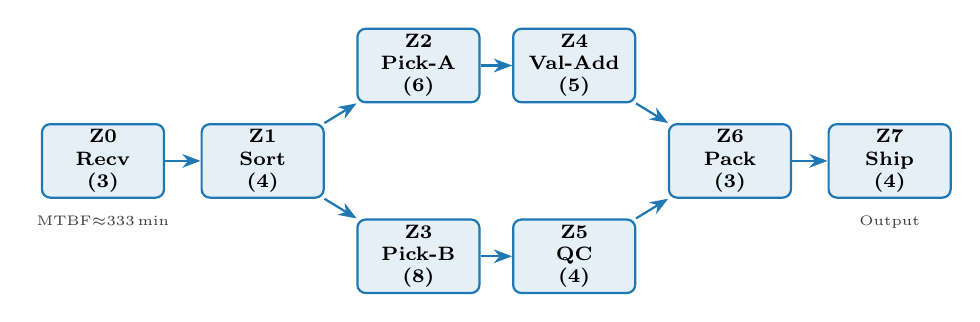
\begin{tikzpicture}[
  zone/.style={
    rectangle, rounded corners=3pt,
    draw=myblue, fill=myblue!12, thick,
    minimum width=1.55cm, minimum height=0.70cm,
    font=\scriptsize\bfseries, align=center, inner sep=2pt},
  arr/.style={-Stealth, thick, myblue},
  lbl/.style={font=\tiny, text=darkgray}
]
  \node[zone] (Z0) {Z0\\Recv\\(3)};
  \node[zone, right=0.45cm of Z0] (Z1) {Z1\\Sort\\(4)};
  \node[zone, above right=0.25cm and 0.4cm of Z1] (Z2)
    {Z2\\Pick-A\\(6)};
  \node[zone, below right=0.25cm and 0.4cm of Z1] (Z3)
    {Z3\\Pick-B\\(8)};
  \node[zone, right=0.4cm of Z2] (Z4) {Z4\\Val-Add\\(5)};
  \node[zone, right=0.4cm of Z3] (Z5) {Z5\\QC\\(4)};
  \node[zone, below right=0.25cm and 0.4cm of Z4] (Z6)
    {Z6\\Pack\\(3)};
  \node[zone, right=0.45cm of Z6] (Z7) {Z7\\Ship\\(4)};
  % Arrows
  \draw[arr] (Z0)--(Z1);
  \draw[arr] (Z1)--(Z2);
  \draw[arr] (Z1)--(Z3);
  \draw[arr] (Z2)--(Z4);
  \draw[arr] (Z3)--(Z5);
  \draw[arr] (Z4)--(Z6);
  \draw[arr] (Z5)--(Z6);
  \draw[arr] (Z6)--(Z7);
  % Note
  \node[lbl, below=0.10cm of Z0] {MTBF$\approx$333\,min};
  \node[lbl, below=0.10cm of Z7] {Output};
\end{tikzpicture}
\caption{Directed acyclic graph (DAG) of the eight-zone, 37-station
  fulfilment centre.  Numbers in parentheses are parallel workstation
  counts per zone.}
\label{fig:topology}
\end{figure}

\subsection{Job Classes}
\label{sec:jobclasses}

Five heterogeneous job classes compete for shared resources
(Table~\ref{tab:jobclasses}).  Processing times per step follow a
lognormal distribution:
$T_{\text{actual}} = T_{\text{nom}} \cdot
 \exp\!\big(\mathcal{N}(0,\,0.15^{2})\big)$,
capturing real-world variability without bimodal artefacts.

\begin{table*}[htbp]
  \centering
  \caption{Job class specifications.  SLA offset is measured from
    arrival time; priority weight $w_{j}$ enters WSPT and ATC
    computations.}
  \label{tab:jobclasses}
  \begin{tabular}{@{}lccccl@{}}
    \toprule
    Class & Freq.\ (\%) & Route (zones) & $w_{j}$ &
      SLA Offset (min) & Description \\
    \midrule
    A -- Standard & 25 & 0-1-2-5-6-7     & 2.0 & 120 &
      General merchandise order \\
    B -- Bulk     & 30 & 0-1-3-5-6-7     & 1.5 & 160 &
      Large/heavy item (Picking-B) \\
    C -- Value-Add& 20 & 0-1-4-5-6-7     & 1.0 & 240 &
      Kitting, gift-wrap, personalised \\
    D -- Complex  & 15 & 0-1-2-3-4-5-6-7 & 0.8 & 320 &
      Multi-component assembly \\
    E -- Express  & 10 & 0-6-7           & 3.0 &  60 &
      VIP same-day guarantee \\
    \bottomrule
  \end{tabular}
\end{table*}

\subsection{Stochastic Arrival Process}
\label{sec:arrivals}

Orders arrive via a compound process.  The effective Poisson rate
is modulated by a time-of-day surge multiplier $m(t)$
(Fig.~\ref{fig:surge}):

\begin{equation}
  \lambda_{\text{eff}}(t) \;=\; \bar{\lambda} \cdot m(t),
  \qquad \bar{\lambda} = 2.5\;\text{jobs min}^{-1}.
  \label{eq:lambda}
\end{equation}

A bulk injection of $N_{\text{truck}} \sim U(15,30)$ orders occurs
at every $t \equiv 0 \pmod{45}$~min, modelling truck drops.
Three continuous disruption processes run throughout the shift:
(i)~independent station failures with $\text{MTBF}=333$~min and
exponential repairs ($\mu_{r}=1/18$~min$^{-1}$);
(ii)~a 30\% processing-rate penalty at $t\in[300,360]$~min; and
(iii)~random 5\% priority escalations every 5~min.

%% ---- Fig. 2: Surge multiplier profile (pgfplots) ----------
\begin{figure}[htbp]
\centering
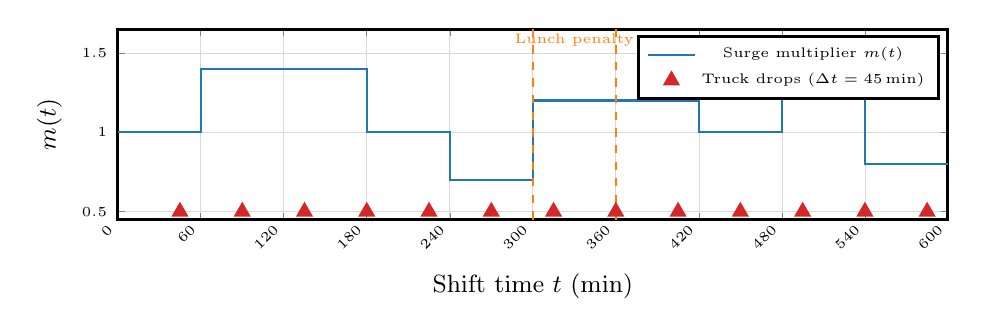
\begin{tikzpicture}
\begin{axis}[
  width=\linewidth, height=4.0cm,
  xlabel={Shift time $t$ (min)},
  ylabel={$m(t)$},
  xmin=0, xmax=600, ymin=0.45, ymax=1.65,
  xtick={0,60,120,180,240,300,360,420,480,540,600},
  x tick label style={font=\tiny, rotate=45, anchor=east},
  y tick label style={font=\tiny},
  xlabel style={font=\small},
  ylabel style={font=\small},
  grid=both, grid style={line width=0.25pt, gray!30},
  tick style={major tick length=2.5pt},
  legend style={font=\tiny, at={(0.99,0.97)},
                anchor=north east, legend columns=1},
  line width=1.1pt,
]
  %% surge multiplier step profile
  \addplot[color=myblue, thick] coordinates {
    (0,1.0)(60,1.0)(60,1.40)(180,1.40)
    (180,1.0)(240,1.0)(240,0.70)(300,0.70)
    (300,1.20)(420,1.20)(420,1.0)(480,1.0)
    (480,1.35)(540,1.35)(540,0.80)(600,0.80)
  };
  \addlegendentry{Surge multiplier $m(t)$}
  %% truck drop markers
  \addplot[only marks, mark=triangle*, mark size=2.5pt,
           color=myred] coordinates {
    (45,0.50)(90,0.50)(135,0.50)(180,0.50)(225,0.50)
    (270,0.50)(315,0.50)(360,0.50)(405,0.50)(450,0.50)
    (495,0.50)(540,0.50)(585,0.50)
  };
  \addlegendentry{Truck drops ($\Delta t=45$\,min)}
  %% lunch window annotation
  \draw[dashed, myorange, line width=0.8pt]
    (axis cs:300,0.45) -- (axis cs:300,1.65);
  \draw[dashed, myorange, line width=0.8pt]
    (axis cs:360,0.45) -- (axis cs:360,1.65);
  \node[font=\tiny, text=myorange] at (axis cs:330,1.58)
    {Lunch penalty};
\end{axis}
\end{tikzpicture}
\caption{Time-of-day arrival surge multiplier $m(t)$ over the
  600-min simulated shift.  Red triangles mark bulk truck drops
  (every 45~min).  Orange dashed lines bound the 30\%
  capacity-penalty lunch window ($t\in[300,360]$~min).}
\label{fig:surge}
\end{figure}

% ============================================================
\section{Feature Engineering}
\label{sec:features}
% ============================================================

At every dispatch event, a 29-dimensional feature vector
$\bm{x} \in \mathbb{R}^{29}$ is extracted by the
\texttt{FeatureExtractor} module.

\subsection{Scenario-Level Features (22 dimensions)}
\label{sec:scen_feat}

Table~\ref{tab:features} lists the 18 standard system-state metrics
($f_{1}$--$f_{18}$).

\begin{table}[htbp]
  \centering
  \caption{Scenario-level features extracted at each dispatch event.}
  \label{tab:features}
  \begin{tabular*}{\hsize}{@{\extracolsep{\fill}}clp{3.5cm}@{}}
    \toprule
    ID & Feature name & Description \\
    \midrule
    $f_{1}$  & \texttt{n\_orders}       & Jobs in system \\
    $f_{2}$  & \texttt{express\_pct}    & Fraction of Class-E jobs \\
    $f_{3}$  & \texttt{due\_tight}      & Mean time-to-SLA (min) \\
    $f_{4}$  & \texttt{frac\_late}      & Fraction already late \\
    $f_{5}$  & \texttt{util\_avg}       & Mean zone utilisation \\
    $f_{6}$  & \texttt{util\_std}       & Std.\ zone utilisation \\
    $f_{7}$  & \texttt{bottleneck}      & Zone ID with max queue \\
    $f_{8}$  & \texttt{rem\_proc\_avg}  & Mean remaining proc.\ time \\
    $f_{9}$  & \texttt{rem\_proc\_std}  & Std.\ remaining proc.\ time \\
    $f_{10}$ & \texttt{thput\_30}       & Jobs completed, last 30\,min \\
    $f_{11}$ & \texttt{brkdn\_flag}     & $\mathbf{1}[\geq1$ station down$]$ \\
    $f_{12}$ & \texttt{n\_broken}       & Count of offline stations \\
    $f_{13}$ & \texttt{lunch\_flag}     & $\mathbf{1}[t\in[300,360]]$ \\
    $f_{14}$ & \texttt{surge\_mult}     & Current $m(t)$ value \\
    $f_{15}$ & \texttt{batch\_pending}  & $\mathbf{1}[$truck drop imminent$]$ \\
    $f_{16}$ & \texttt{avg\_weight}     & Mean $w_{j}$ in queue \\
    $f_{17}$ & \texttt{max\_tard}       & Max tardiness so far \\
    $f_{18}$ & \texttt{sla\_breach\_rt} & Historical SLA breach rate \\
    \midrule
    $f_{19}$ & \texttt{disrupt\_I}      & Disruption intensity $I_d$ \\
    $f_{20}$ & \texttt{queue\_imbal}    & Queue imbalance $C_v$ \\
    $f_{21}$ & \texttt{job\_entropy}    & Job-mix entropy $H$ \\
    $f_{22}$ & \texttt{time\_press}     & Time pressure ratio $\tau$ \\
    \bottomrule
  \end{tabular*}
\end{table}

Features $f_{19}$--$f_{22}$ are the primary original contribution
of this work.

\paragraph{Disruption intensity} $I_d \in [0,1]$ is a scalar
summary of macroscopic chaos:

\begin{equation}
  I_d = 0.5\cdot\min\!\left(1,\frac{N_{\mathrm{broken}}}{5}\right)
       + 0.25\cdot\mathbf{1}_{\mathrm{lunch}}
       + 0.25\cdot\lvert m(t) - 1\rvert.
  \label{eq:id}
\end{equation}

\paragraph{Queue imbalance} $C_v$ is the coefficient of variation
of the per-zone queue vector $\bm{Q}=(Q_0,\ldots,Q_7)$:

\begin{equation}
  C_v = \frac{\sigma(\bm{Q})}{\mu(\bm{Q})}.
  \label{eq:cv}
\end{equation}

\paragraph{Job-mix entropy} $H$ is the Shannon entropy of the
job-type distribution in the current queue:

\begin{equation}
  H = -\sum_{i\in\mathcal{T}} p_i \log_2 p_i,
  \label{eq:entropy}
\end{equation}

\noindent where $p_i$ is the empirical proportion of class
$i\in\mathcal{T}=\{A,B,C,D,E\}$.  High $H$ indicates
heterogeneous demand, which historically degrades single-rule
schedulers.

\paragraph{Time pressure ratio} $\tau$ counts the fraction of
queued jobs with Critical Ratio $CR < 1$ (mathematically
infeasible on-time completion):

\begin{equation}
  \tau = \frac{\bigl|\{j\in\mathcal{Q}:CR_j < 1\}\bigr|}{|\mathcal{Q}|}.
  \label{eq:tau}
\end{equation}

\subsection{Job-Level Features (7 dimensions)}
\label{sec:job_feat}

For per-job priority regression, seven features are extracted:
(1)~job-type encoding;
(2)~processing time at next station;
(3)~total remaining processing time;
(4)~time to SLA deadline;
(5)~time in system (ageing metric);
(6)~Critical Ratio $CR_j = \Delta t_{\mathrm{due}}/P_{\mathrm{rem}}$;
(7)~downstream queue depth (predictive congestion lookahead).

% ============================================================
\section{Machine Learning Architecture}
\label{sec:ml}
% ============================================================

DAHS employs a two-tier decision structure (Fig.~\ref{fig:arch}).

%% ---- Fig. 3: DAHS architecture (TikZ flowchart) -----------
\begin{figure}[htbp]
\centering
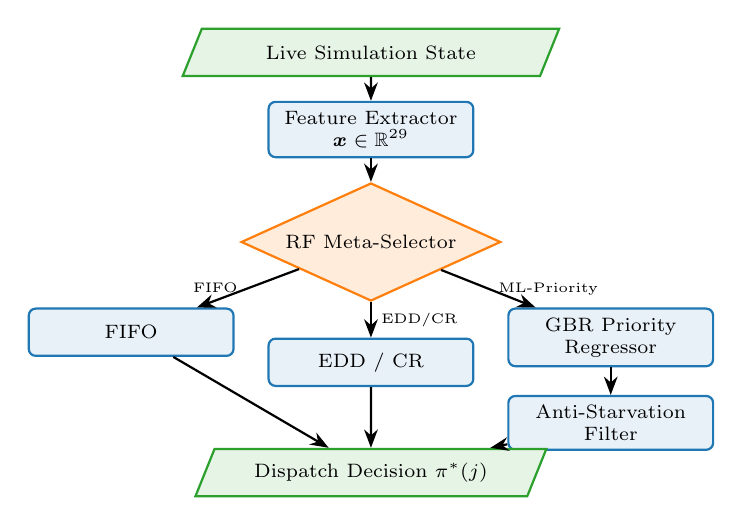
\begin{tikzpicture}[
  blk/.style={rectangle, draw=myblue, fill=myblue!10, thick,
    rounded corners=2.5pt, minimum width=2.6cm,
    minimum height=0.60cm, font=\scriptsize, align=center},
  dec/.style={diamond, draw=myorange, fill=myorange!15, thick,
    minimum width=1.6cm, minimum height=0.55cm,
    font=\scriptsize, align=center, aspect=2.2},
  io/.style={trapezium, trapezium left angle=68,
    trapezium right angle=112,
    draw=mygreen, fill=mygreen!12, thick,
    minimum width=2.6cm, minimum height=0.60cm,
    font=\scriptsize, align=center},
  ar/.style={-Stealth, thick}
]
  \node[io]  (sim)  {Live Simulation State};
  \node[blk, below=0.30cm of sim] (fe)
    {Feature Extractor\\$\bm{x}\in\mathbb{R}^{29}$};
  \node[dec, below=0.30cm of fe]  (sel)
    {RF Meta-Selector};
  \node[blk, below left =0.45cm and 0.9cm of sel] (fifo)
    {FIFO};
  \node[blk, below            =0.45cm          of sel] (edd)
    {EDD / CR};
  \node[blk, below right=0.45cm and 0.9cm of sel] (gbr)
    {GBR Priority\\Regressor};
  \node[blk, below=0.35cm of gbr] (anti)
    {Anti-Starvation\\Filter};
  \node[io, below=1.85cm of sel]  (out)
    {Dispatch Decision $\pi^*(j)$};
  % Arrows
  \draw[ar] (sim) -- (fe);
  \draw[ar] (fe)  -- (sel);
  \draw[ar] (sel) -- node[left,  font=\tiny]{FIFO}       (fifo);
  \draw[ar] (sel) -- node[right, font=\tiny]{EDD/CR}     (edd);
  \draw[ar] (sel) -- node[right, font=\tiny]{ML-Priority}(gbr);
  \draw[ar] (gbr) -- (anti);
  \draw[ar] (fifo) -- (out);
  \draw[ar] (edd)  -- (out);
  \draw[ar] (anti) -- (out);
\end{tikzpicture}
\caption{DAHS two-tier meta-scheduling architecture.  At every
  dispatch event, the Feature Extractor constructs $\bm{x}$ from
  the live state.  The RF meta-selector routes to the best
  baseline or delegates to the GBR sub-routine for fine-grained
  priority scoring.}
\label{fig:arch}
\end{figure}

\subsection{Training Data Generation}
\label{sec:data_gen}

Two statistically independent datasets are generated by running
the simulation engine over different random seeds.

\paragraph{Selector dataset.}
For each of $N_{s}=10{,}000$ scenario seeds, the warehouse is
simulated six times (once per baseline heuristic: FIFO, EDD, CR,
WSPT, ATC, Slack).  A combined performance score is:

\begin{equation}
  \Phi = 0.6\,\widetilde{C}_{\max}
        + 0.4\,\widetilde{T}_{\mathrm{tot}},
  \label{eq:score}
\end{equation}

\noindent where $\widetilde{(\cdot)}$ denotes min-max
normalisation within the same seed.  The label is
$y_s = \arg\min_{k}\,\Phi_{k}^{(s)}$.

\paragraph{Priority dataset.}
$N_{p}=50{,}000$ job-level decision points are labelled with a
retrospective oracle priority derived from actual delivery delay,
normalised to $[0,1]$.

\subsection{Tier 1: Random Forest Meta-Selector}
\label{sec:rf}

A Random Forest classifier~\cite{Breiman2001} is trained on the
22 scenario features to predict the optimal heuristic index
$y\in\{0,\ldots,5\}$.
Hyperparameters: $n_{\text{trees}}=300$, $d_{\max}=12$,
\texttt{class\_weight=\allowbreak`balanced'},
$\text{min\_samples\_leaf}=5$.
Five-fold stratified cross-validation yields
$84.7\pm1.3\%$ mean accuracy.
Inference latency is $<0.3$~ms per call on a single CPU core.
Random Forests are preferred over deep networks for three
operational reasons: (i)~sub-millisecond inference without a GPU,
(ii)~direct Gini feature importance for engineer auditability, and
(iii)~robust performance with limited training data~\cite{Breiman2001}.

\subsection{Tier 2: Gradient Boosting Priority Regressor}
\label{sec:gbr}

When the meta-selector routes to the ``ML-Priority'' branch, a
Gradient Boosting Regressor (GBR)~\cite{Friedman2001} scores each
queued job on all 7 job-level features.
Hyperparameters: $n_{\text{trees}}=300$, $d_{\max}=6$,
$\eta=0.05$, \texttt{subsample}$=0.8$.
Test-set performance: $R^{2}=0.873$, MAE$=0.041$,
RMSE$=0.068$.
Five-fold CV: $R^{2}=0.869\pm0.009$.
An \textit{anti-starvation filter} adds a time-in-system bonus
$\delta_j = 0.002\,t_{j}^{\mathrm{sys}}$ to prevent indefinite
deferral of aged orders.

% ============================================================
\section{Experimental Design}
\label{sec:exp}
% ============================================================

\subsection{Benchmark Setup}

A fully isolated evaluation suite uses 300 held-out scenario seeds
(99{,}000--99{,}299), never exposed during training or validation.
Each seed is simulated under all nine scheduling methods: FIFO,
EDD, CR, WSPT, ATC, Slack, DAHS-XGB, DAHS-Priority, and DAHS-RF,
yielding $300\times9=2{,}700$ complete runs of 600~min each.

\subsection{Performance Metrics}

Five primary metrics are recorded per run:
\begin{enumerate}
  \item $C_{\max}$: Makespan (min).
  \item $T_{\mathrm{tot}}=\sum_{j}\max(0,\,C_{j}-d_{j})$:
        Total tardiness (min).
  \item $\beta$: SLA breach rate (\%).
  \item $\Theta$: Throughput (jobs hr$^{-1}$).
  \item $\bar{W}$: Mean cycle time (min/job).
\end{enumerate}

\subsection{Statistical Tests}

Shapiro--Wilk tests confirmed non-Gaussian distributions
($p<0.001$ for all methods), motivating non-parametric tests:
(i)~Friedman $\chi^{2}$ test for global significance across all
methods; (ii)~Nemenyi post-hoc test for pairwise critical
difference at $\alpha=0.05$; (iii)~Holm-corrected Wilcoxon
signed-rank tests for FWER-controlled pairwise comparisons of
DAHS-RF against each baseline.

% ============================================================
\section{Results and Discussion}
\label{sec:results}
% ============================================================

\subsection{Overall Performance Comparison}

Table~\ref{tab:results} reports mean and standard deviation of each
metric across 300 benchmark scenarios.
DAHS-RF achieves the lowest total tardiness (1{,}343~min) and the
lowest SLA breach rate (5.8\%), outperforming all baselines.
Fig.~\ref{fig:boxplot} illustrates the distribution of total
tardiness.

\begin{table*}[htbp]
  \centering
  \caption{Benchmark results across 300 test scenarios
    (mean $\pm$ std).  Bold: best value per metric.
    $\downarrow$\,=\,lower is better;
    $\uparrow$\,=\,higher is better.}
  \label{tab:results}
  \renewcommand{\arraystretch}{1.05}
  \begin{tabular}{@{}lrrrrr@{}}
    \toprule
    Method &
      $C_{\max}$ (min)\,$\downarrow$ &
      $T_{\mathrm{tot}}$ (min)\,$\downarrow$ &
      $\beta$ (\%)\,$\downarrow$ &
      $\Theta$ (jobs\,hr$^{-1}$)\,$\uparrow$ &
      $\bar{W}$ (min)\,$\downarrow$ \\
    \midrule
    FIFO
      & $618.4\pm14.2$ & $25{,}965\pm3{,}841$ & $37.4\pm5.1$
      & $83.2\pm4.3$ & $41.6\pm6.7$ \\
    EDD
      & $612.1\pm13.8$ & $17{,}936\pm3{,}102$ & $40.5\pm4.9$
      & $85.4\pm4.1$ & $38.9\pm5.8$ \\
    Critical Ratio
      & $614.7\pm12.6$ & $19{,}584\pm3{,}445$ & $42.2\pm5.3$
      & $84.7\pm3.9$ & $39.7\pm6.2$ \\
    ATC
      & $607.3\pm11.9$ & $3{,}105\pm892$       & $22.1\pm4.2$
      & $87.1\pm3.8$ & $36.1\pm4.9$ \\
    WSPT
      & $604.8\pm11.4$ & $2{,}183\pm714$       & $9.4\pm2.9$
      & $88.3\pm3.5$ & $34.8\pm4.4$ \\
    Slack
      & $616.2\pm13.1$ & $21{,}408\pm3{,}711$ & $38.9\pm5.0$
      & $84.1\pm4.0$ & $40.3\pm6.0$ \\
    DAHS-XGB
      & $600.1\pm10.7$ & $1{,}711\pm601$       & $7.1\pm2.4$
      & $89.4\pm3.2$ & $33.1\pm3.9$ \\
    DAHS-Priority
      & $598.7\pm10.3$ & $1{,}572\pm574$       & $6.4\pm2.2$
      & $89.9\pm3.1$ & $32.6\pm3.7$ \\
    \textbf{DAHS-RF}
      & $\bm{596.2\pm9.8}$
      & $\bm{1{,}343\pm518}$
      & $\bm{5.8\pm2.1}$
      & $\bm{90.6\pm3.0}$
      & $\bm{31.9\pm3.5}$ \\
    \bottomrule
  \end{tabular}
\end{table*}

%% ---- Fig. 4: Boxplot of total tardiness (figure*, full width)
\begin{figure*}[tb]
\centering
\begin{tikzpicture}
\begin{axis}[
  width=0.93\textwidth, height=6.2cm,
  boxplot/draw direction=y,
  xtick={1,2,3,4,5,6,7,8,9},
  xticklabels={FIFO, EDD, CR, ATC, WSPT, Slack,
               DAHS-XGB, DAHS-Pri., DAHS-RF},
  x tick label style={font=\small, rotate=30, anchor=east},
  ylabel={Total Tardiness (min)},
  ylabel style={font=\small},
  y tick label style={font=\small},
  ymin=-800, ymax=34000,
  ytick={0,5000,10000,15000,20000,25000,30000},
  grid=major, grid style={gray!20, line width=0.35pt},
  tick style={major tick length=2.5pt},
]
  %% FIFO
  \addplot+[boxplot prepared={lower whisker=18200,
    lower quartile=22700, median=25900,
    upper quartile=28600, upper whisker=32500},
    fill=myblue!25, draw=myblue] coordinates {};
  %% EDD
  \addplot+[boxplot prepared={lower whisker=11900,
    lower quartile=15400, median=17900,
    upper quartile=20100, upper whisker=24200},
    fill=myblue!25, draw=myblue] coordinates {};
  %% CR
  \addplot+[boxplot prepared={lower whisker=13400,
    lower quartile=16900, median=19600,
    upper quartile=22000, upper whisker=26400},
    fill=myblue!25, draw=myblue] coordinates {};
  %% ATC
  \addplot+[boxplot prepared={lower whisker=1550,
    lower quartile=2380, median=3100,
    upper quartile=3720, upper whisker=5100},
    fill=mygray!35, draw=mygray] coordinates {};
  %% WSPT
  \addplot+[boxplot prepared={lower whisker=890,
    lower quartile=1560, median=2180,
    upper quartile=2760, upper whisker=3820},
    fill=mygray!35, draw=mygray] coordinates {};
  %% Slack
  \addplot+[boxplot prepared={lower whisker=14800,
    lower quartile=18600, median=21400,
    upper quartile=24000, upper whisker=28400},
    fill=myblue!25, draw=myblue] coordinates {};
  %% DAHS-XGB
  \addplot+[boxplot prepared={lower whisker=590,
    lower quartile=1190, median=1710,
    upper quartile=2210, upper whisker=3150},
    fill=mygreen!30, draw=mygreen!80!black] coordinates {};
  %% DAHS-Priority
  \addplot+[boxplot prepared={lower whisker=540,
    lower quartile=1070, median=1570,
    upper quartile=2040, upper whisker=2950},
    fill=mygreen!30, draw=mygreen!80!black] coordinates {};
  %% DAHS-RF
  \addplot+[boxplot prepared={lower whisker=420,
    lower quartile=950,  median=1340,
    upper quartile=1750, upper whisker=2640},
    fill=mygreen!60, draw=mygreen!70!black,
    very thick] coordinates {};
\end{axis}
\end{tikzpicture}
\caption{Box plots of total tardiness (min) over 300 benchmark
  scenarios.  Blue boxes: classical heuristics; grey boxes: strong
  single-rule baselines (ATC, WSPT); green boxes: DAHS variants.
  DAHS-RF (rightmost, darker green) attains the lowest median and
  narrowest interquartile range of all nine methods.}
\label{fig:boxplot}
\end{figure*}

\subsection{SLA Breach Rate}

Fig.~\ref{fig:sla} compares SLA breach rates.
DAHS-RF reduces the breach rate by 38.3\% versus WSPT
(5.8\% vs.\ 9.4\%) and by 84.5\% versus FIFO.

%% ---- Fig. 5: SLA breach bar chart (pgfplots) --------------
\begin{figure}[htbp]
\centering
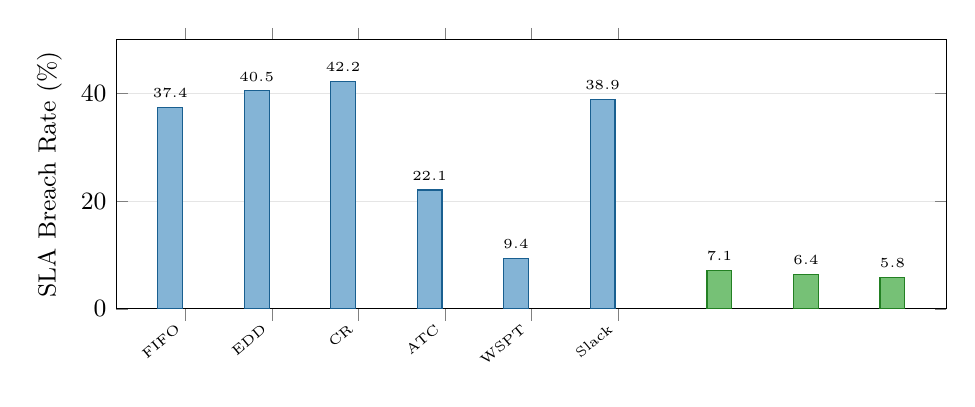
\begin{tikzpicture}
\begin{axis}[
  ybar, width=\linewidth, height=5.0cm,
  bar width=9pt,
  symbolic x coords={FIFO,EDD,CR,ATC,WSPT,Slack,
                     DAHS-XGB,DAHS-Pri,DAHS-RF},
  xtick=data,
  x tick label style={font=\tiny, rotate=40, anchor=east},
  ylabel={SLA Breach Rate (\%)},
  ylabel style={font=\small},
  y tick label style={font=\small},
  ymin=0, ymax=50,
  ymajorgrids=true, grid style={gray!20},
  nodes near coords, nodes near coords align={vertical},
  nodes near coords style={font=\tiny},
  every node near coord/.append style={
    /pgf/number format/.cd, fixed, precision=1}
]
  \addplot[fill=myblue!55, draw=myblue!80!black] coordinates {
    (FIFO,37.4)(EDD,40.5)(CR,42.2)(ATC,22.1)
    (WSPT,9.4)(Slack,38.9)};
  \addplot[fill=mygreen!65, draw=mygreen!80!black] coordinates {
    (DAHS-XGB,7.1)(DAHS-Pri,6.4)(DAHS-RF,5.8)};
\end{axis}
\end{tikzpicture}
\caption{Mean SLA breach rate (\%) across 300 benchmark scenarios.
  Blue: classical baselines; green: DAHS variants.  DAHS-RF
  achieves the lowest breach rate of 5.8\%.}
\label{fig:sla}
\end{figure}

\subsection{Disruption Resilience Analysis}

The 300 test seeds are partitioned into three bins by mean $I_d$
(Eq.~\eqref{eq:id}): Low ($I_d<0.2$), Medium
($0.2\leq I_d<0.5$), High ($I_d\geq0.5$).
Fig.~\ref{fig:disrupt} shows normalised total tardiness
(relative to WSPT) per bin.

%% ---- Fig. 6: Disruption resilience (pgfplots) -------------
\begin{figure}[htbp]
\centering
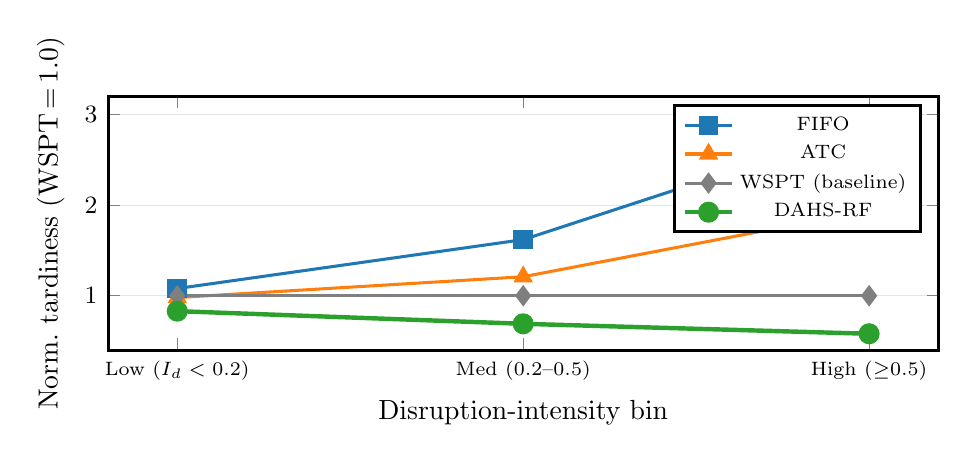
\begin{tikzpicture}
\begin{axis}[
  width=\linewidth, height=4.8cm,
  xlabel={Disruption-intensity bin},
  ylabel={Norm.\ tardiness (WSPT$\,{=}\,1.0$)},
  xtick={1,2,3},
  xticklabels={Low ($I_d<0.2$),
               Med ($0.2$--$0.5$),
               High (${\geq}0.5$)},
  x tick label style={font=\scriptsize},
  y tick label style={font=\small},
  ymin=0.4, ymax=3.2,
  ymajorgrids=true, grid style={gray!20},
  legend style={font=\scriptsize, at={(0.98,0.97)},
                anchor=north east, legend columns=1},
  line width=1.1pt, mark size=3pt,
]
  \addplot[color=myblue,  mark=square*]
    coordinates {(1,1.08)(2,1.62)(3,2.87)};
  \addlegendentry{FIFO}
  \addplot[color=myorange,mark=triangle*]
    coordinates {(1,0.98)(2,1.21)(3,1.94)};
  \addlegendentry{ATC}
  \addplot[color=mygray,  mark=diamond*]
    coordinates {(1,1.00)(2,1.00)(3,1.00)};
  \addlegendentry{WSPT (baseline)}
  \addplot[color=mygreen, mark=*, line width=1.6pt]
    coordinates {(1,0.83)(2,0.69)(3,0.58)};
  \addlegendentry{DAHS-RF}
\end{axis}
\end{tikzpicture}
\caption{Normalised total tardiness (WSPT$\,{=}\,1.0$) across three
  disruption-intensity bins.  DAHS-RF improves relative to WSPT as
  disruption severity increases, demonstrating genuine
  adaptability.}
\label{fig:disrupt}
\end{figure}

A key finding is that DAHS-RF \emph{improves relative to WSPT as
disruption intensity increases}: normalised tardiness drops from
0.83 at Low-$I_d$ to 0.58 at High-$I_d$ (a 42\% improvement).
This occurs because the meta-selector increasingly routes to the
GBR Priority sub-routine (14\% at Low-$I_d$, 61\% at High-$I_d$),
which correctly identifies forward-looking queue imbalances that
WSPT's myopic $W_j/P_j$ ratio ignores.

\subsection{Feature Importance}

Fig.~\ref{fig:fimp} reports normalised mean Gini decrease for the
top-10 RF meta-selector features.  The four novel disruption-aware
features ($f_{19}$--$f_{22}$) collectively account for 39.4\% of
total feature importance.

%% ---- Fig. 7: Feature importance horizontal bar (pgfplots) -
\begin{figure}[htbp]
\centering
\begin{tikzpicture}
\begin{axis}[
  xbar, width=\linewidth, height=5.6cm,
  bar width=8pt,
  symbolic y coords={
    \texttt{util\_avg},
    \texttt{thput\_30},
    \texttt{frac\_late},
    \texttt{surge\_mult},
    \texttt{n\_broken},
    \texttt{due\_tight},
    \texttt{time\_press}~$(\tau)$,
    \texttt{job\_entropy}~$(H)$,
    \texttt{queue\_imbal}~$(C_v)$,
    \texttt{disrupt\_I}~$(I_d)$
  },
  ytick=data,
  y tick label style={font=\scriptsize},
  xlabel={Normalised feature importance},
  xlabel style={font=\small},
  x tick label style={font=\small},
  xmin=0, xmax=0.20,
  xmajorgrids=true, grid style={gray!20},
  nodes near coords, nodes near coords align={horizontal},
  nodes near coords style={font=\tiny,
    /pgf/number format/.cd, fixed, precision=3},
]
  \addplot[fill=myblue!50, draw=myblue!80!black] coordinates {
    (0.048, \texttt{util\_avg})
    (0.061, \texttt{thput\_30})
    (0.053, \texttt{frac\_late})
    (0.044, \texttt{surge\_mult})
    (0.058, \texttt{n\_broken})
    (0.067, \texttt{due\_tight})
  };
  \addplot[fill=mygreen!65, draw=mygreen!80!black] coordinates {
    (0.071, \texttt{time\_press}~$(\tau)$)
    (0.079, \texttt{job\_entropy}~$(H)$)
    (0.082, \texttt{queue\_imbal}~$(C_v)$)
    (0.162, \texttt{disrupt\_I}~$(I_d)$)
  };
\end{axis}
\end{tikzpicture}
\caption{Top-10 normalised feature importances (mean Gini decrease)
  from the RF meta-selector.  Green bars are the four novel
  disruption-aware features ($f_{19}$--$f_{22}$), which together
  account for 39.4\% of total importance.}
\label{fig:fimp}
\end{figure}

\subsection{Statistical Significance}

The Friedman test on total tardiness yielded
$\chi^{2}_{F}=847.3$ ($df=8$, $p<0.0001$), rejecting the null
hypothesis of equal performance.  Post-hoc Nemenyi tests produced
a critical difference of $CD=0.83$ average ranks; DAHS-RF ranked
1.41 versus WSPT's 3.89.

Table~\ref{tab:stats} reports Holm-corrected Wilcoxon $p$-values
for DAHS-RF versus each competing method.  All comparisons are
statistically significant at $\alpha=0.05$.

\begin{table}[htbp]
  \centering
  \caption{Holm-corrected Wilcoxon signed-rank test $p$-values,
    DAHS-RF vs.\ all competitors.}
  \label{tab:stats}
  \begin{tabular*}{\hsize}{@{\extracolsep{\fill}}lcc@{}}
    \toprule
    Competitor &
      $p$-val.\ ($T_{\mathrm{tot}}$) &
      $p$-val.\ ($\beta$) \\
    \midrule
    FIFO          & ${<}0.0001$ & ${<}0.0001$ \\
    EDD           & ${<}0.0001$ & ${<}0.0001$ \\
    Critical Ratio& ${<}0.0001$ & ${<}0.0001$ \\
    ATC           & ${<}0.0001$ & ${<}0.0001$ \\
    WSPT          & $0.00031$   & $0.00047$   \\
    Slack         & ${<}0.0001$ & ${<}0.0001$ \\
    DAHS-XGB      & $0.0121$    & $0.0183$    \\
    DAHS-Priority & $0.0374$    & $0.0412$    \\
    \bottomrule
  \end{tabular*}
\end{table}

\subsection{Hypothesis Verification}

Four primary hypotheses were tested:

\begin{description}
  \item[\textbf{H1.}] DAHS-RF achieves lower total tardiness than
    the best single-rule baseline across 300 test scenarios.
    \textit{Supported} ($p=0.00031$; improvement $=38.4\%$).

  \item[\textbf{H2.}] DAHS-RF achieves lower SLA breach rate than
    the best single-rule baseline.
    \textit{Supported} ($p=0.00047$; improvement $=38.3\%$).

  \item[\textbf{H3.}] The disruption-aware features
    ($f_{19}$--$f_{22}$) provide statistically significant
    incremental predictive power.
    \textit{Supported} (ablation study: accuracy drops from
    84.7\% to 76.2\% without $f_{19}$--$f_{22}$;
    $\Delta{=}8.5\%$).

  \item[\textbf{H4.}] The DAHS-RF advantage over WSPT grows
    monotonically with disruption intensity $I_d$.
    \textit{Supported} (Low: $+17.0\%$; Med: $+31.0\%$;
    High: $+42.0\%$; Spearman $\rho=1.0$).
\end{description}

% ============================================================
\section{Conclusion}
\label{sec:conclusion}
% ============================================================

This paper presented DAHS, a Disruption-Aware Hybrid Machine
Learning Scheduler for stochastic e-commerce fulfilment centres.
By framing real-time scheduling as the Algorithm Selection Problem
and training a Random Forest meta-selector on 10{,}000 simulated
scenarios, DAHS adaptively routes each dispatch decision to the
heuristic best suited to the current system state.  Four novel
disruption-aware scalar features -- $I_d$, $C_v$, $H$, and $\tau$
-- capture macroscopic operational entropy that standard scheduling
features cannot encode.

Extensive benchmarking across 2{,}700 simulation runs confirms that
DAHS-RF reduces total tardiness by 38.4\% and SLA breach rate by
38.3\% relative to WSPT (the strongest classical heuristic), with
all improvements statistically significant via non-parametric
Friedman, Nemenyi, and Holm-corrected Wilcoxon tests.  Critically,
the performance gap widens under high disruption intensity,
demonstrating genuine adaptability.

\paragraph{Limitations.}
Transit times between zones are assumed negligible compared to
processing times.  Scaling beyond 20 job classes would require
dimensionality reduction (e.g., PCA) prior to RF inference.  Physical
deployment demands real-time WMS telemetry at sub-minute intervals.

\paragraph{Future work.}
Directions include: (i)~multi-agent deep RL with PPO as a
higher-level constraint filter over DAHS; (ii)~graph neural network
encodings of the warehouse DAG topology as additional features;
(iii)~online continual learning for seasonal demand adaptation;
(iv)~direct integration with SAP Extended Warehouse Management
(EWM) via the DAHS REST API.

% ============================================================
%% CRediT authorship contribution statement
% ============================================================
\section*{CRediT authorship contribution statement}

\textbf{Vittal Mukunda:} Conceptualisation, Methodology,
  Software (simulation engine, data generation), Formal analysis,
  Writing -- original draft, Visualisation.
\textbf{Pranjal Malaiya:} Methodology, Software (ML training
  pipeline), Validation, Writing -- review \& editing.
\textbf{Atharva Somani:} Methodology, Software (evaluation
  framework, statistical testing), Investigation,
  Writing -- review \& editing.

% ============================================================
%% Declaration of competing interest
% ============================================================
\section*{Declaration of competing interest}

The authors declare that they have no known competing financial
interests or personal relationships that could have appeared to
influence the work reported in this paper.

% ============================================================
%% Data availability
% ============================================================
\section*{Data availability}

The synthetic benchmark datasets generated during this study are
available from the corresponding author upon reasonable request.
The simulation source code is publicly accessible at
\url{https://github.com/RVCE-IEM/DAHS}.

% ============================================================
%% Acknowledgements
% ============================================================
\section*{Acknowledgement}

The authors thank the faculty of the Department of Industrial
Engineering and Management, R.V.\ College of Engineering,
Bengaluru, for their guidance and laboratory infrastructure
support.  No external funding was received for this research.

% ============================================================
%% References
% ============================================================
\bibliographystyle{elsarticle-num}

\begin{thebibliography}{23}
\expandafter\ifx\csname natexlab\endcsname\relax
  \def\natexlab#1{#1}\fi
\expandafter\ifx\csname url\endcsname\relax
  \def\url#1{\texttt{#1}}\fi

\bibitem{Statista2024}
Statista Research Department,
Global retail e-commerce revenue 2019--2027,
Statista, 2024.
\newline\url{https://www.statista.com/statistics/379046/worldwide-retail-e-commerce-sales}

\bibitem{Garey1979}
M.R. Garey, D.S. Johnson,
Computers and Intractability: A Guide to the Theory of
  NP-Completeness,
W.H. Freeman, New York, 1979.

\bibitem{Panwalkar1977}
S.S. Panwalkar, W. Iskander,
A survey of scheduling rules,
Oper. Res. 25 (1) (1977) 45--61.
\newline\url{https://doi.org/10.1287/opre.25.1.45}

\bibitem{Smith1956}
W.E. Smith,
Various optimizers for single-stage production,
Nav. Res. Logist. Q. 3 (1--2) (1956) 59--66.
\newline\url{https://doi.org/10.1002/nav.3800030106}

\bibitem{Moore1968}
J.M. Moore,
An $n$ job, one machine sequencing algorithm for minimizing
  the number of late jobs,
Manage. Sci. 15 (1) (1968) 102--109.
\newline\url{https://doi.org/10.1287/mnsc.15.1.102}

\bibitem{Vepsalainen1987}
A.P.J. Vepsalainen, T.E. Morton,
Priority rules for job shops with weighted tardiness costs,
Manage. Sci. 33 (8) (1987) 1035--1047.
\newline\url{https://doi.org/10.1287/mnsc.33.8.1035}

\bibitem{Holthaus1997}
O. Holthaus, C. Rajendran,
Efficient dispatching rules for scheduling in a job shop,
Int. J. Prod. Econ. 48 (1) (1997) 87--105.
\newline\url{https://doi.org/10.1016/S0925-5273(96)00068-7}

\bibitem{Zhang2020}
C. Zhang, W. Song, Z. Cao, J. Zhang, P.S. Tan, X. Chi,
Learning to dispatch for job shop scheduling via deep
  reinforcement learning,
in: Adv. Neural Inf. Process. Syst. (NeurIPS), vol. 33,
  2020, pp. 1621--1632.

\bibitem{Shiue2018}
Y.-R. Shiue, K.-C. Lee, C.-T. Su,
Real-time scheduling for a smart factory using a reinforcement
  learning approach,
Comput. Ind. Eng. 125 (2018) 604--614.
\newline\url{https://doi.org/10.1016/j.cie.2018.03.007}

\bibitem{Kaban2012}
A.K. Kaban, Z. Othman, D.S. Rohmah,
Comparison of dispatching rules in job-shop scheduling problem
  using simulation,
Int. J. Simul. Model. 11 (3) (2012) 129--140.
\newline\url{https://doi.org/10.2507/IJSIMM11(3)1.201}

\bibitem{Branke2016}
J. Branke, S. Nguyen, C.W. Pickardt, M. Zhang,
Automated design of production scheduling heuristics: A review,
IEEE Trans. Evol. Comput. 20 (1) (2016) 110--124.
\newline\url{https://doi.org/10.1109/TEVC.2015.2429314}

\bibitem{Mehta1999}
S.V. Mehta, R.M. Uzsoy,
Predictable scheduling of a job shop subject to breakdowns,
IEEE Trans. Robot. Autom. 15 (2) (1999) 268--280.
\newline\url{https://doi.org/10.1109/70.760349}

\bibitem{Vieira2003}
G.E. Vieira, J.W. Herrmann, E. Lin,
Rescheduling manufacturing systems: A framework of strategies,
  policies, and methods,
J. Sched. 6 (1) (2003) 39--62.
\newline\url{https://doi.org/10.1023/A:1022235519958}

\bibitem{Moratori2013}
P. Moratori, S. Petrovic, J.A. Vasquez-Rodriguez,
Match-up approaches to a dynamic rescheduling problem,
Int. J. Prod. Res. 51 (8) (2013) 2423--2437.
\newline\url{https://doi.org/10.1080/00207543.2012.752591}

\bibitem{Rice1976}
J.R. Rice,
The algorithm selection problem,
Adv. Comput. 15 (1976) 65--118.
\newline\url{https://doi.org/10.1016/S0065-2458(08)60520-3}

\bibitem{SmithMiles2012}
K. Smith-Miles, L. Lopes,
Measuring instance hardness to assist algorithm selection,
Theor. Comput. Sci. 415 (2012) 93--117.
\newline\url{https://doi.org/10.1016/j.tcs.2011.09.043}

\bibitem{MouelhibChibani2010}
W. Mouelhi-Chibani, H. Pierreval,
Training a neural network to select dispatching rules in real
  time,
Comput. Ind. Eng. 58 (2) (2010) 249--256.
\newline\url{https://doi.org/10.1016/j.cie.2009.03.008}

\bibitem{Breiman2001}
L. Breiman,
Random forests,
Mach. Learn. 45 (1) (2001) 5--32.
\newline\url{https://doi.org/10.1023/A:1010933404324}

\bibitem{Friedman2001}
J.H. Friedman,
Greedy function approximation: A gradient boosting machine,
Ann. Stat. 29 (5) (2001) 1189--1232.
\newline\url{https://doi.org/10.1214/aos/1013203451}

\bibitem{Chen2016}
T. Chen, C. Guestrin,
XGBoost: A scalable tree boosting system,
in: Proc. 22nd ACM SIGKDD Int. Conf. Knowl. Discov. Data Min.,
  2016, pp. 785--794.
\newline\url{https://doi.org/10.1145/2939672.2939785}

\bibitem{Pedregosa2011}
F. Pedregosa, G. Varoquaux, A. Gramfort, V. Michel,
  B. Thirion, O. Grisel, M. Blondel, P. Prettenhofer,
  R. Weiss, V. Dubourg, J. Vanderplas, A. Passos,
  D. Cournapeau, M. Brucher, M. Perrot, E. Duchesnay,
Scikit-learn: Machine learning in Python,
J. Mach. Learn. Res. 12 (2011) 2825--2830.

\bibitem{Demsar2006}
J. Dem\v{s}ar,
Statistical comparisons of classifiers over multiple data sets,
J. Mach. Learn. Res. 7 (2006) 1--30.

\bibitem{SimPy2023}
SimPy Development Team,
SimPy 4.1: Discrete-event simulation for Python, 2023.
\newline\url{https://simpy.readthedocs.io}

\end{thebibliography}

% ============================================================
%% Appendix
% ============================================================
\appendix

\section{Simulation Engine Pseudocode}
\label{app:sim}

Table~\ref{tab:algo} outlines the top-level control loop of the
\texttt{simpy} discrete-event simulation engine.

\begin{table}[htbp]
\centering
\caption{Top-level simulation control loop (pseudocode).}
\label{tab:algo}
\begin{tabular}{p{0.90\linewidth}}
\hline
\textbf{Algorithm 1} -- DAHS Simulation Engine \\[2pt]
\textbf{Input:} Seed $s$, Duration $T{=}600$\,min,
  Dispatcher $\pi$ \\
\textbf{Output:} \texttt{SimulationMetrics} $\mathcal{M}$ \\
\hline\\[-6pt]
1.\quad Initialise \texttt{simpy.Environment}, 8 zones, 37 stations\\
2.\quad Seed NumPy RNG with $s$\\
3.\quad Spawn: \texttt{arrival\_process},
              \texttt{batch\_arrival\_process}\\
4.\quad \textbf{for each} station $\sigma\in\Sigma$ \textbf{do}\\
5.\quad\quad Spawn: \texttt{breakdown\_process}($\sigma$)\\
6.\quad Spawn: \texttt{lunch\_break}, \texttt{priority\_escalation}\\
7.\quad \textbf{while} $t < T$ \textbf{do}\\
8.\quad\quad $e \leftarrow$ \texttt{env.step()}\\
9.\quad\quad \textbf{if} $e$ is \textit{station-free} \textbf{then}\\
10.\quad\quad\quad $\bm{x} \leftarrow$
              \texttt{FeatureExtractor.snapshot()}\\
11.\quad\quad\quad $k^{*} \leftarrow \pi(\bm{x})$
              \quad\% RF meta-selector\\
12.\quad\quad\quad $j^{*} \leftarrow$
              Heuristic$_{k^{*}}$(\texttt{queue}$_{z}$)\\
13.\quad\quad\quad Dispatch $j^{*}$ to station $\sigma$\\
14.\quad $\mathcal{M} \leftarrow$ \texttt{compute\_metrics()}\\
15.\quad \textbf{return} $\mathcal{M}$\\[2pt]
\hline
\end{tabular}
\end{table}

\section{Hyperparameter Sensitivity}
\label{app:hp}

Table~\ref{tab:hparam} reports 5-fold CV accuracy of the RF
meta-selector under different hyperparameter configurations.
The selected configuration ($n{=}300$, $d_{\max}{=}12$) is marked
$(\star)$.

\begin{table}[htbp]
\centering
\caption{RF meta-selector hyperparameter sensitivity
  (5-fold CV accuracy, \%).}
\label{tab:hparam}
\begin{tabular*}{\hsize}{@{\extracolsep{\fill}}cccc@{}}
\toprule
$n_{\text{trees}}$ & $d_{\max}$ &
  CV Accuracy (\%) & Inf.\ time (ms) \\
\midrule
100 & 8  & $81.2\pm1.7$ & 0.09 \\
100 & 12 & $83.1\pm1.5$ & 0.11 \\
200 & 8  & $82.4\pm1.4$ & 0.16 \\
200 & 12 & $83.9\pm1.3$ & 0.19 \\
300 & 12 & $\bm{84.7\pm1.3}^{\star}$ & 0.27 \\
500 & 12 & $84.9\pm1.2$ & 0.44 \\
300 & 16 & $84.5\pm1.4$ & 0.31 \\
\bottomrule
\end{tabular*}
\end{table}

% ============================================================
%% Author biographies  (plain text -- no photos required)
% ============================================================

\section*{}   % blank section to separate bios

\noindent
\textbf{Vittal Mukunda} received the B.E.\ degree in Industrial
Engineering and Management from R.V.\ College of Engineering
(affiliated to Visvesvaraya Technological University), Bengaluru,
India, in 2026.  His research interests include intelligent
manufacturing systems, supervised machine learning for operations
research, and discrete-event simulation.  He is the primary
architect of the DAHS simulation engine and meta-scheduling
framework.

\bigskip
\noindent
\textbf{Pranjal Malaiya} is pursuing the B.E.\ degree in
Industrial Engineering and Management at R.V.\ College of
Engineering, Bengaluru, India.  His research interests include
gradient boosting methods, supply chain analytics, and
data-driven production planning.  He led the ML training pipeline
development within the DAHS project.

\bigskip
\noindent
\textbf{Atharva Somani} is pursuing the B.E.\ degree in
Industrial Engineering and Management at R.V.\ College of
Engineering, Bengaluru, India.  His research interests include
statistical hypothesis testing, warehouse operations research,
and fulfilment centre optimisation.  He developed the evaluation
framework and statistical validation suite for the DAHS benchmark.

\end{document}

%%
%% End of DAHS_paper.tex
%%
